\documentclass{article}%
\usepackage[T1]{fontenc}%
\usepackage[utf8]{inputenc}%
\usepackage{lmodern}%
\usepackage{textcomp}%
\usepackage{lastpage}%
\usepackage{geometry}%
\geometry{margin=0.7in}%
\usepackage{ragged2e}%
\usepackage{graphicx}%
\usepackage{enumitem}%
\usepackage{fancyhdr}%
%
\fancypagestyle{header}{%
\renewcommand{\headrulewidth}{0pt}%
\renewcommand{\footrulewidth}{0pt}%
\fancyhead{%
}%
\fancyfoot{%
}%
\fancyhead[L]{%
Universite Cergy Pontoise%
\linebreak%
irenee.briquel@gmail.com%
}%
\fancyhead[C]{%
Annee 2021%
}%
\fancyhead[R]{%
Automates et langages reguliers%
\linebreak%
L2%
}%
}%
%
\begin{document}%
\normalsize%
\pagestyle{header}%
\begin{minipage}{\textwidth}%
\centering%
\begin{Large}%
\textbf{Examen de deuxieme session {-} Langages et automates}%
\end{Large}%
\linebreak%
\begin{large}%
\textbf{Mardi 12 juin 2018}%
\end{large}%
\end{minipage}%
\section{Exercice 1}%
\label{sec:Exercice1}%
\subsection{Soit l'automate suivant:}%
\label{subsec:Soitlautomatesuivant}%


\begin{figure}[h!]%
\centering%
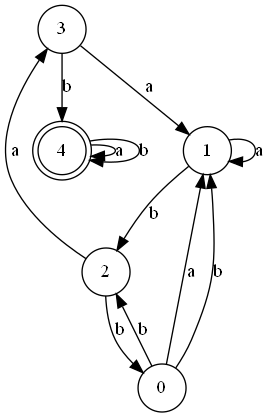
\includegraphics[width=120px]{./../Results/abab.png}%
\end{figure}

%
\begin{enumerate}[label=\alph*),start=20]%
\item%
Trouver l'automate deterministe.%
\item%
Trouver l'automate minimal.%
\end{enumerate}

%
\end{document}